\documentclass[11pt]{article}
\usepackage[english]{babel}
\usepackage[utf8]{inputenc}
\usepackage{fancyhdr}
\usepackage{graphicx}

\def\Name{Ran Liao}
\def\Topic{Team}

\title{\textbf{\Topic}}
\author{\Name}
\markboth{Notes on \Topic\ }{Notes on \Topic\ }
\date{\today}
 
\pagestyle{fancy}
\fancyhf{}
\rhead{\date{\today} }
\lhead{Notes on \Topic\ }
\rfoot{\thepage}

\textheight=9in
%\textwidth=6.5in
\topmargin=-.75in
%\oddsidemargin=0in
%\evensidemargin=0in
 
\begin{document}
\maketitle
\noindent\makebox[\linewidth]{\rule[8pt]{5in}{0.5pt}}

\section*{Democratic Team}

The basic concept under this approach is called ``Egoless Programming". Because if programmers are highly attached to their code, they may see their modules as extension of themselves and even name their modules after themselves. As a result, he/she may be unwilling to find all the errors in his/her code. One proposed solution to this problem is egoless programming, including

\begin{itemize}
	\item Restructure the social environment
	\item Restructure programmers' values
	\item Encourage team members to find faults in code
	\item A fault must be considered a normal and accepted event
	\item The team as whole will develop an ethos, a group identity
	\item Modules will ``belong" to the team as whole
	\item A group of up to 10 egoless programmers constitutes a democratic team
\end{itemize}

\begin{figure}[h]
	\centering
	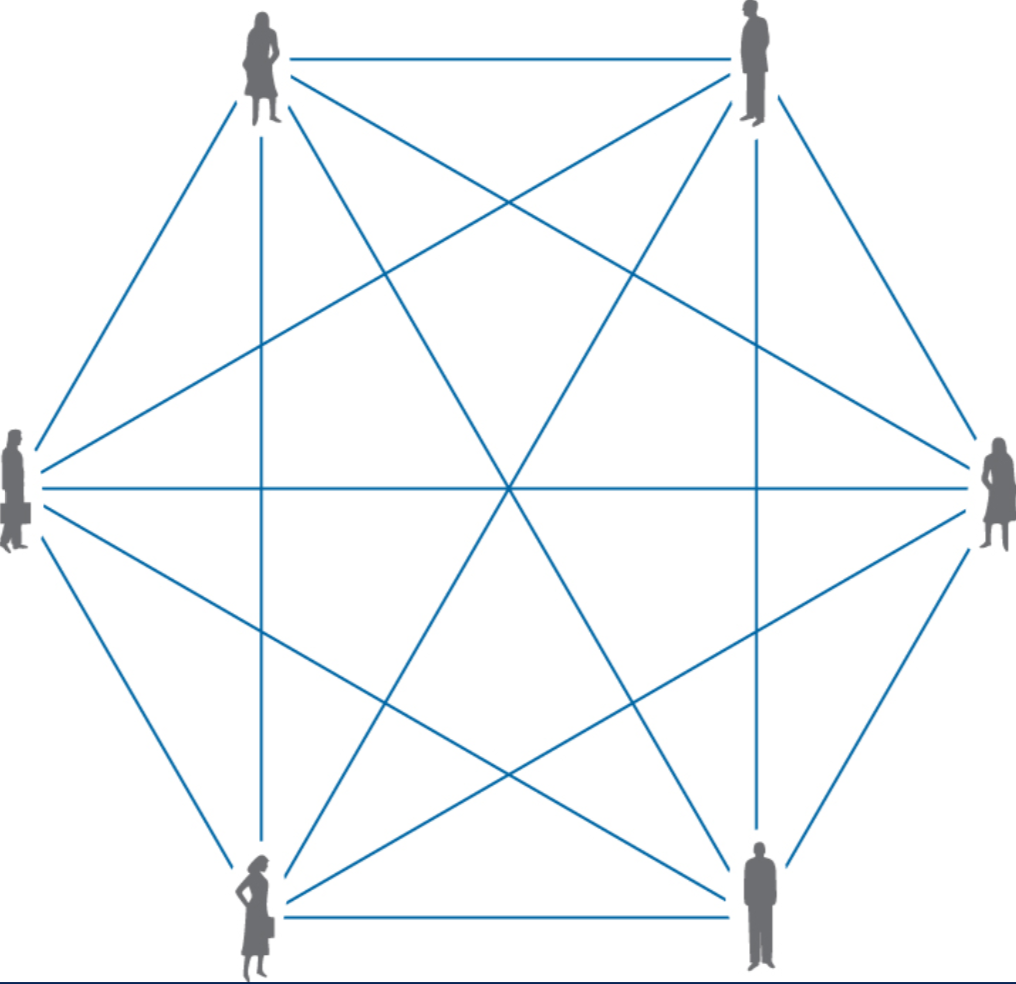
\includegraphics[width=0.4\linewidth]{images/DemocraticTeam.png}
	\caption{Democratic Team}
	\label{fig:DemocraticTeam}
\end{figure}


\section*{Chief Programmer Team}

This approach focus on specialization and hierarchy. Each role has its one responsibility.

\begin{figure}[h]
	\centering
	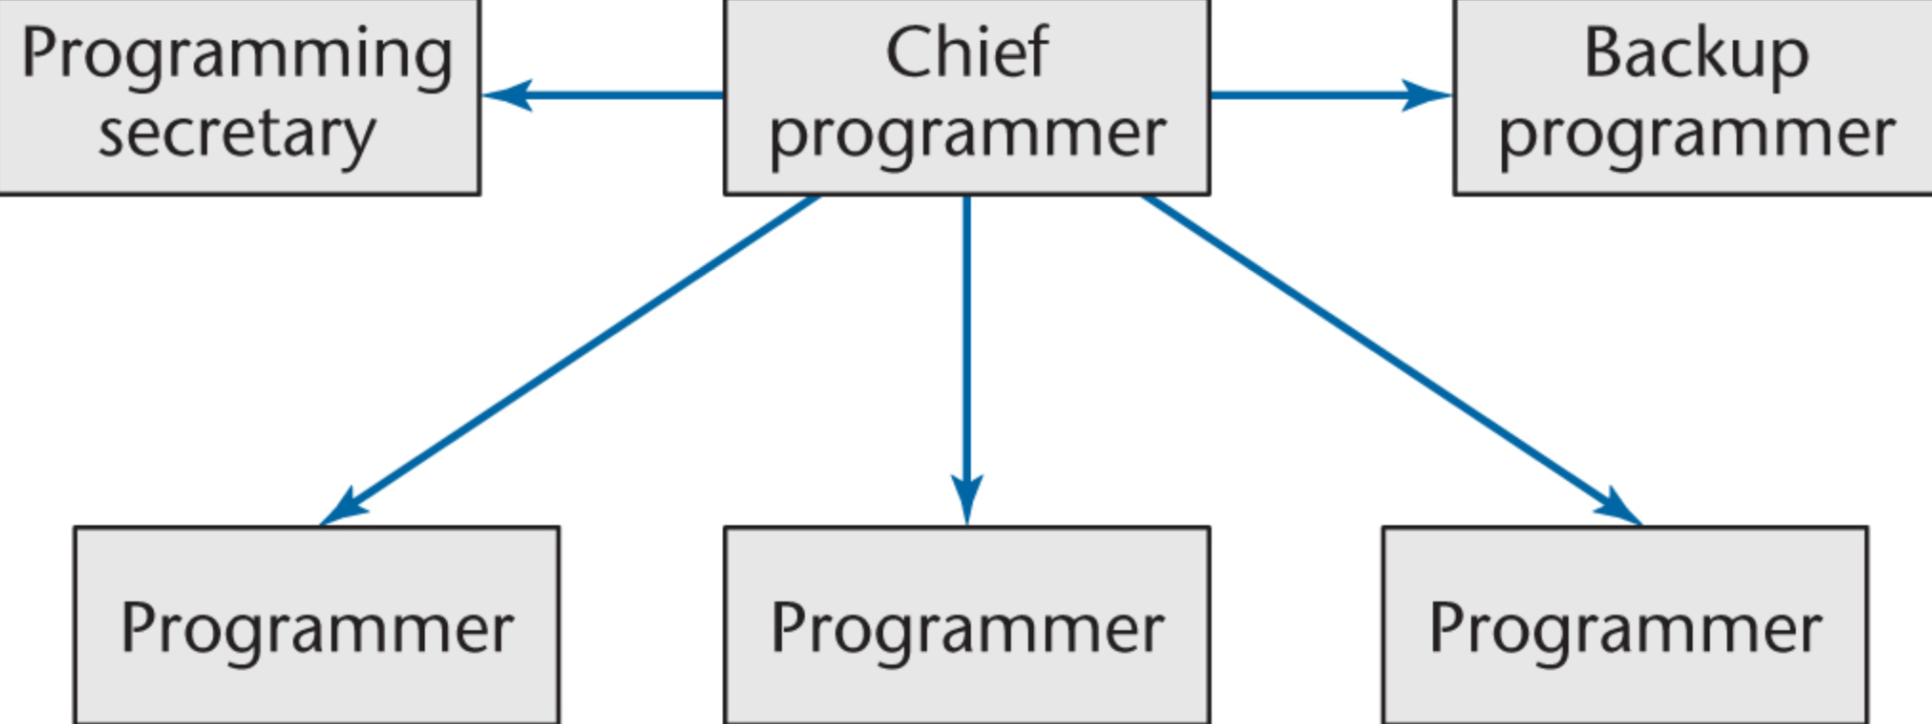
\includegraphics[width=0.9\linewidth]{images/ChiefProgrammerTeam.png}
	\caption{Chief Programmer Team}
	\label{fig:ChiefProgrammerTeam}
\end{figure}





\end{document}